\documentclass[screen, aspectratio=43]{beamer}
\usepackage[T1]{fontenc}
\usepackage[utf8]{inputenc}
\usepackage{xcolor}
\usepackage{listings}
\newcommand{\CPP}[0]{{C\nolinebreak[4]\hspace{-.1em}\raisebox{.1ex}{\small\bf +\hspace{-.1em}+\ }}}

\newcommand{\gfcb}[1]{%
    \fcolorbox{white}{gray!10!}{\quad\strut #1\quad}
    } % gfcb := gray fcolorbox

\usepackage{pgfpages}

\usepackage{gnuplottex} %miktex option if using miktex on windows

% Notes page for presentation with pympress
\setbeamertemplate{note page}[plain]
%Comment the next line out for standard pdf without notes
\setbeameroption{show notes on second screen=right}

% Use the NTNU-temaet for beamer 
% \usetheme[style=ntnu|simple|vertical|horizontal, 
%     language=bm|nn|en, smalltitle, 
%     city=all|trondheim|alesund|gjovik]{ntnu2017}
\usetheme[style=simple,language=en]{ntnu2017}


\usepackage[english]{babel}
\usepackage[style=numeric,backend=biber,natbib=false,sorting=none]{biblatex}
\usepackage{csvsimple}  % for simple table reading and display

\usepackage{booktabs}

\title[Latex Document]{Why use Latex to create \\Documents at NTNU}
\subtitle{Using the Beamer class}
\author[S. McCallum]{Simon McCallum}
\institute[NTNU]{Department of Computer Sciences, NTNU}
\date{06 April 2020}
%\date{} % To have an empty date

\addbibresource{example.bib} % Add bibliography database

% Set the reference style to numeric.
% See here: http://tex.stackexchange.com/questions/68080/beamer-bibliography-icon
\setbeamertemplate{bibliography item}[text] 

% Set bibliography fonts to a small size.
\renewcommand*{\bibfont}{\footnotesize}


\begin{document}
%-----------------------------------------
\begin{frame}
  \titlepage
\end{frame}

% Alternatively, special title page command to get a different background
% \ntnutitlepage

%-----------------------------------------
\begin{frame}
  \frametitle{Content vs Style}
  \begin{itemize}
      \item {\LaTeX} deals with formatting so you don't have to.
      \item Learn Latex in 30 minutes: \url{https://www.overleaf.com/learn/latex/Learn_LaTeX_in_30_minutes}
      \item Markup language based on describing \emph{content}
      \item Uses a container "begin" and "end" model for describing behaviour.
      \item Numbering things, referencing things, deciding where things go?
      \item Your tool influences your focus
  \end{itemize}
    \note{Discuss links to learning on the Overleaf in 30 minutes\\
    Give examples of markup languages like HTML\\
    Separation of display and content}
\end{frame}

%-----------------------------------------
\begin{frame}
  \frametitle{Formatting}
  \begin{itemize}
      \item You are unlikely to be an expert at layout
      \item Journals, Conferences have required formats
      \item Web content - CSS changes display of HTML
      \item Citation formats - so many standards!
      \item Contents page, Appendix, References, Abstracts ........
      \item Invest time early to save time later.
  \end{itemize}
\end{frame}


%-----------------------------------------
\begin{frame}
  \frametitle{Sharing}
  \begin{itemize}
      \item Overleaf - like google docs for latex
      \item Save as text files - easy sharing
      \item Works with version control tools
      \item No hidden content in your editor
      \item Write in separate text files
      \item Your words express your thoughts - your thoughts are important!
  \end{itemize}
\end{frame}

%-----------------------------------------
\begin{frame}
  \frametitle{Including files}
  \begin{itemize}
      \item Include as many tex files by name as you like
      \item allows logical separation of content
      \item Use file system structure to help you
      \item \gfcb{\detokenize{\include{inc/structure}}}
      \item compile only parts of the document
      \item create reusable content
  \end{itemize}
    \note{Structure to help organisation\\
   examples\\
    }
\end{frame}

%-----------------------------------------
\begin{frame}
  \frametitle{Including Images}
   \noindent
 \parbox[t]{.75\textwidth}{
  \begin{itemize}
      \item Standard figure includes - do the tutorial
      \item Numbering figures so you can refer to them
      \item Using the figure environment
  \end{itemize}}
     \hfill
       \raisebox{-.5\height}{
     \includegraphics[width=.2\textwidth]{beamerthementnu2017/figures/kart_student}}
  \begin{itemize}
      \item include \gfcb{\detokenize{\caption[short text contents page]{text...}}}
      \item All Figures must appear with text reference
      \item \gfcb{\detokenize{\includegraphics[width=.2\textwidth]{figures/kart_student}}}
  \end{itemize}    
    \note{
    
    }
\end{frame}


%-----------------------------------------
\begin{frame}
  \frametitle{Citations}
  \begin{itemize}
      \item Using \gfcb{.bib} file to store information
      \item Download citations in bibtex format from online paper Databases
      \item Record abstracts and notes next to reference
      \item Uses the id from the bibtex file
      \item Can use multiple .bib files
      \item Two styles at NTNU, Harvard and Vancouver.  \\
      \gfcb{\detokenize{\setboolean{HarvardCitations}{false}}}
      \item CS uses Vancouver and so you set Harvard to false \\
      \gfcb{\detokenize{~\cite{Askvall1985}}}
  \end{itemize}
  
    \note{
   
    }

\end{frame}

%-----------------------------------------
\begin{frame}[fragile]
  \frametitle{Citations}
  \begin{lstlisting}[breaklines]
  @misc{latex2005,
  title={A beginner's introduction to typesetting with LATEX},
  author={Flynn, Peter},
  year={2005},
  url={http://ctan.ijs.si/tex-archive/documentation/beginlatex/src/old/beginlatex.letter.pdf}
  \end{lstlisting}
\end{frame}

%-----------------------------------------
\begin{frame}
  \frametitle{Charts}
  \begin{itemize}
      \item Include as graphics
      \item gnuplot creates nice Latex charts
      \item Use an integrated format psTricks   
      \item Option to compile graphics inline
      \item Create from a csv file
      \item Scripting for large numbers of charts
      \item Including Latex math in charts
  \end{itemize}
    \note{
  
    }
\end{frame}

%-----------------------------------------
\begin{frame}
  \frametitle{Gnuplot}

\begin{figure}[htp]  %t top, b bottom, p page | you can also use h to try to get the figure to appear at the current location
  \centering
  \scalebox{.7}{% GNUPLOT: LaTeX picture
\setlength{\unitlength}{0.240900pt}
\ifx\plotpoint\undefined\newsavebox{\plotpoint}\fi
\begin{picture}(1500,900)(0,0)
\sbox{\plotpoint}{\rule[-0.200pt]{0.400pt}{0.400pt}}%
\put(130.0,82.0){\rule[-0.200pt]{4.818pt}{0.400pt}}
\put(110,82){\makebox(0,0)[r]{-1}}
\put(1419.0,82.0){\rule[-0.200pt]{4.818pt}{0.400pt}}
\put(130.0,151.0){\rule[-0.200pt]{4.818pt}{0.400pt}}
\put(110,151){\makebox(0,0)[r]{-0.8}}
\put(1419.0,151.0){\rule[-0.200pt]{4.818pt}{0.400pt}}
\put(130.0,221.0){\rule[-0.200pt]{4.818pt}{0.400pt}}
\put(110,221){\makebox(0,0)[r]{-0.6}}
\put(1419.0,221.0){\rule[-0.200pt]{4.818pt}{0.400pt}}
\put(130.0,290.0){\rule[-0.200pt]{4.818pt}{0.400pt}}
\put(110,290){\makebox(0,0)[r]{-0.4}}
\put(1419.0,290.0){\rule[-0.200pt]{4.818pt}{0.400pt}}
\put(130.0,360.0){\rule[-0.200pt]{4.818pt}{0.400pt}}
\put(110,360){\makebox(0,0)[r]{-0.2}}
\put(1419.0,360.0){\rule[-0.200pt]{4.818pt}{0.400pt}}
\put(130.0,429.0){\rule[-0.200pt]{4.818pt}{0.400pt}}
\put(110,429){\makebox(0,0)[r]{ 0}}
\put(1419.0,429.0){\rule[-0.200pt]{4.818pt}{0.400pt}}
\put(130.0,498.0){\rule[-0.200pt]{4.818pt}{0.400pt}}
\put(110,498){\makebox(0,0)[r]{ 0.2}}
\put(1419.0,498.0){\rule[-0.200pt]{4.818pt}{0.400pt}}
\put(130.0,568.0){\rule[-0.200pt]{4.818pt}{0.400pt}}
\put(110,568){\makebox(0,0)[r]{ 0.4}}
\put(1419.0,568.0){\rule[-0.200pt]{4.818pt}{0.400pt}}
\put(130.0,637.0){\rule[-0.200pt]{4.818pt}{0.400pt}}
\put(110,637){\makebox(0,0)[r]{ 0.6}}
\put(1419.0,637.0){\rule[-0.200pt]{4.818pt}{0.400pt}}
\put(130.0,707.0){\rule[-0.200pt]{4.818pt}{0.400pt}}
\put(110,707){\makebox(0,0)[r]{ 0.8}}
\put(1419.0,707.0){\rule[-0.200pt]{4.818pt}{0.400pt}}
\put(130.0,776.0){\rule[-0.200pt]{4.818pt}{0.400pt}}
\put(110,776){\makebox(0,0)[r]{ 1}}
\put(1419.0,776.0){\rule[-0.200pt]{4.818pt}{0.400pt}}
\put(130.0,82.0){\rule[-0.200pt]{0.400pt}{4.818pt}}
\put(130,41){\makebox(0,0){-10}}
\put(130.0,756.0){\rule[-0.200pt]{0.400pt}{4.818pt}}
\put(457.0,82.0){\rule[-0.200pt]{0.400pt}{4.818pt}}
\put(457,41){\makebox(0,0){-5}}
\put(457.0,756.0){\rule[-0.200pt]{0.400pt}{4.818pt}}
\put(785.0,82.0){\rule[-0.200pt]{0.400pt}{4.818pt}}
\put(785,41){\makebox(0,0){ 0}}
\put(785.0,756.0){\rule[-0.200pt]{0.400pt}{4.818pt}}
\put(1112.0,82.0){\rule[-0.200pt]{0.400pt}{4.818pt}}
\put(1112,41){\makebox(0,0){ 5}}
\put(1112.0,756.0){\rule[-0.200pt]{0.400pt}{4.818pt}}
\put(1439.0,82.0){\rule[-0.200pt]{0.400pt}{4.818pt}}
\put(1439,41){\makebox(0,0){ 10}}
\put(1439.0,756.0){\rule[-0.200pt]{0.400pt}{4.818pt}}
\put(130.0,82.0){\rule[-0.200pt]{0.400pt}{167.185pt}}
\put(130.0,82.0){\rule[-0.200pt]{315.338pt}{0.400pt}}
\put(1439.0,82.0){\rule[-0.200pt]{0.400pt}{167.185pt}}
\put(130.0,776.0){\rule[-0.200pt]{315.338pt}{0.400pt}}
\put(784,838){\makebox(0,0){Test of $y=sin(x)$}}
\put(785,429){\makebox(0,0)[l]{$y=sin(x)$}}
\put(1279,736){\makebox(0,0)[r]{sin(x)}}
\put(1299.0,736.0){\rule[-0.200pt]{24.090pt}{0.400pt}}
\put(130,618){\usebox{\plotpoint}}
\multiput(130.58,609.67)(0.493,-2.439){23}{\rule{0.119pt}{2.008pt}}
\multiput(129.17,613.83)(13.000,-57.833){2}{\rule{0.400pt}{1.004pt}}
\multiput(143.58,546.90)(0.493,-2.677){23}{\rule{0.119pt}{2.192pt}}
\multiput(142.17,551.45)(13.000,-63.450){2}{\rule{0.400pt}{1.096pt}}
\multiput(156.58,479.28)(0.494,-2.553){25}{\rule{0.119pt}{2.100pt}}
\multiput(155.17,483.64)(14.000,-65.641){2}{\rule{0.400pt}{1.050pt}}
\multiput(170.58,408.77)(0.493,-2.717){23}{\rule{0.119pt}{2.223pt}}
\multiput(169.17,413.39)(13.000,-64.386){2}{\rule{0.400pt}{1.112pt}}
\multiput(183.58,340.15)(0.493,-2.598){23}{\rule{0.119pt}{2.131pt}}
\multiput(182.17,344.58)(13.000,-61.577){2}{\rule{0.400pt}{1.065pt}}
\multiput(196.58,274.92)(0.493,-2.360){23}{\rule{0.119pt}{1.946pt}}
\multiput(195.17,278.96)(13.000,-55.961){2}{\rule{0.400pt}{0.973pt}}
\multiput(209.58,216.42)(0.494,-1.892){25}{\rule{0.119pt}{1.586pt}}
\multiput(208.17,219.71)(14.000,-48.709){2}{\rule{0.400pt}{0.793pt}}
\multiput(223.58,165.35)(0.493,-1.607){23}{\rule{0.119pt}{1.362pt}}
\multiput(222.17,168.17)(13.000,-38.174){2}{\rule{0.400pt}{0.681pt}}
\multiput(236.58,125.75)(0.493,-1.171){23}{\rule{0.119pt}{1.023pt}}
\multiput(235.17,127.88)(13.000,-27.877){2}{\rule{0.400pt}{0.512pt}}
\multiput(249.58,97.67)(0.493,-0.576){23}{\rule{0.119pt}{0.562pt}}
\multiput(248.17,98.83)(13.000,-13.834){2}{\rule{0.400pt}{0.281pt}}
\put(262,83.17){\rule{2.700pt}{0.400pt}}
\multiput(262.00,84.17)(7.396,-2.000){2}{\rule{1.350pt}{0.400pt}}
\multiput(275.00,83.58)(0.582,0.492){21}{\rule{0.567pt}{0.119pt}}
\multiput(275.00,82.17)(12.824,12.000){2}{\rule{0.283pt}{0.400pt}}
\multiput(289.58,95.00)(0.493,1.012){23}{\rule{0.119pt}{0.900pt}}
\multiput(288.17,95.00)(13.000,24.132){2}{\rule{0.400pt}{0.450pt}}
\multiput(302.58,121.00)(0.493,1.527){23}{\rule{0.119pt}{1.300pt}}
\multiput(301.17,121.00)(13.000,36.302){2}{\rule{0.400pt}{0.650pt}}
\multiput(315.58,160.00)(0.493,1.924){23}{\rule{0.119pt}{1.608pt}}
\multiput(314.17,160.00)(13.000,45.663){2}{\rule{0.400pt}{0.804pt}}
\multiput(328.58,209.00)(0.494,2.113){25}{\rule{0.119pt}{1.757pt}}
\multiput(327.17,209.00)(14.000,54.353){2}{\rule{0.400pt}{0.879pt}}
\multiput(342.58,267.00)(0.493,2.558){23}{\rule{0.119pt}{2.100pt}}
\multiput(341.17,267.00)(13.000,60.641){2}{\rule{0.400pt}{1.050pt}}
\multiput(355.58,332.00)(0.493,2.717){23}{\rule{0.119pt}{2.223pt}}
\multiput(354.17,332.00)(13.000,64.386){2}{\rule{0.400pt}{1.112pt}}
\multiput(368.58,401.00)(0.493,2.757){23}{\rule{0.119pt}{2.254pt}}
\multiput(367.17,401.00)(13.000,65.322){2}{\rule{0.400pt}{1.127pt}}
\multiput(381.58,471.00)(0.493,2.677){23}{\rule{0.119pt}{2.192pt}}
\multiput(380.17,471.00)(13.000,63.450){2}{\rule{0.400pt}{1.096pt}}
\multiput(394.58,539.00)(0.494,2.333){25}{\rule{0.119pt}{1.929pt}}
\multiput(393.17,539.00)(14.000,59.997){2}{\rule{0.400pt}{0.964pt}}
\multiput(408.58,603.00)(0.493,2.241){23}{\rule{0.119pt}{1.854pt}}
\multiput(407.17,603.00)(13.000,53.152){2}{\rule{0.400pt}{0.927pt}}
\multiput(421.58,660.00)(0.493,1.845){23}{\rule{0.119pt}{1.546pt}}
\multiput(420.17,660.00)(13.000,43.791){2}{\rule{0.400pt}{0.773pt}}
\multiput(434.58,707.00)(0.493,1.408){23}{\rule{0.119pt}{1.208pt}}
\multiput(433.17,707.00)(13.000,33.493){2}{\rule{0.400pt}{0.604pt}}
\multiput(447.58,743.00)(0.494,0.827){25}{\rule{0.119pt}{0.757pt}}
\multiput(446.17,743.00)(14.000,21.429){2}{\rule{0.400pt}{0.379pt}}
\multiput(461.00,766.58)(0.652,0.491){17}{\rule{0.620pt}{0.118pt}}
\multiput(461.00,765.17)(11.713,10.000){2}{\rule{0.310pt}{0.400pt}}
\multiput(474.00,774.93)(1.378,-0.477){7}{\rule{1.140pt}{0.115pt}}
\multiput(474.00,775.17)(10.634,-5.000){2}{\rule{0.570pt}{0.400pt}}
\multiput(487.58,768.29)(0.493,-0.695){23}{\rule{0.119pt}{0.654pt}}
\multiput(486.17,769.64)(13.000,-16.643){2}{\rule{0.400pt}{0.327pt}}
\multiput(500.58,748.50)(0.493,-1.250){23}{\rule{0.119pt}{1.085pt}}
\multiput(499.17,750.75)(13.000,-29.749){2}{\rule{0.400pt}{0.542pt}}
\multiput(513.58,715.37)(0.494,-1.599){25}{\rule{0.119pt}{1.357pt}}
\multiput(512.17,718.18)(14.000,-41.183){2}{\rule{0.400pt}{0.679pt}}
\multiput(527.58,669.82)(0.493,-2.083){23}{\rule{0.119pt}{1.731pt}}
\multiput(526.17,673.41)(13.000,-49.408){2}{\rule{0.400pt}{0.865pt}}
\multiput(540.58,615.67)(0.493,-2.439){23}{\rule{0.119pt}{2.008pt}}
\multiput(539.17,619.83)(13.000,-57.833){2}{\rule{0.400pt}{1.004pt}}
\multiput(553.58,553.03)(0.493,-2.638){23}{\rule{0.119pt}{2.162pt}}
\multiput(552.17,557.51)(13.000,-62.514){2}{\rule{0.400pt}{1.081pt}}
\multiput(566.58,486.28)(0.494,-2.553){25}{\rule{0.119pt}{2.100pt}}
\multiput(565.17,490.64)(14.000,-65.641){2}{\rule{0.400pt}{1.050pt}}
\multiput(580.58,415.77)(0.493,-2.717){23}{\rule{0.119pt}{2.223pt}}
\multiput(579.17,420.39)(13.000,-64.386){2}{\rule{0.400pt}{1.112pt}}
\multiput(593.58,347.03)(0.493,-2.638){23}{\rule{0.119pt}{2.162pt}}
\multiput(592.17,351.51)(13.000,-62.514){2}{\rule{0.400pt}{1.081pt}}
\multiput(606.58,280.79)(0.493,-2.400){23}{\rule{0.119pt}{1.977pt}}
\multiput(605.17,284.90)(13.000,-56.897){2}{\rule{0.400pt}{0.988pt}}
\multiput(619.58,220.94)(0.493,-2.043){23}{\rule{0.119pt}{1.700pt}}
\multiput(618.17,224.47)(13.000,-48.472){2}{\rule{0.400pt}{0.850pt}}
\multiput(632.58,170.48)(0.494,-1.562){25}{\rule{0.119pt}{1.329pt}}
\multiput(631.17,173.24)(14.000,-40.242){2}{\rule{0.400pt}{0.664pt}}
\multiput(646.58,128.75)(0.493,-1.171){23}{\rule{0.119pt}{1.023pt}}
\multiput(645.17,130.88)(13.000,-27.877){2}{\rule{0.400pt}{0.512pt}}
\multiput(659.58,100.41)(0.493,-0.655){23}{\rule{0.119pt}{0.623pt}}
\multiput(658.17,101.71)(13.000,-15.707){2}{\rule{0.400pt}{0.312pt}}
\multiput(672.00,84.95)(2.695,-0.447){3}{\rule{1.833pt}{0.108pt}}
\multiput(672.00,85.17)(9.195,-3.000){2}{\rule{0.917pt}{0.400pt}}
\multiput(685.00,83.58)(0.704,0.491){17}{\rule{0.660pt}{0.118pt}}
\multiput(685.00,82.17)(12.630,10.000){2}{\rule{0.330pt}{0.400pt}}
\multiput(699.58,93.00)(0.493,0.972){23}{\rule{0.119pt}{0.869pt}}
\multiput(698.17,93.00)(13.000,23.196){2}{\rule{0.400pt}{0.435pt}}
\multiput(712.58,118.00)(0.493,1.448){23}{\rule{0.119pt}{1.238pt}}
\multiput(711.17,118.00)(13.000,34.430){2}{\rule{0.400pt}{0.619pt}}
\multiput(725.58,155.00)(0.493,1.924){23}{\rule{0.119pt}{1.608pt}}
\multiput(724.17,155.00)(13.000,45.663){2}{\rule{0.400pt}{0.804pt}}
\multiput(738.58,204.00)(0.493,2.241){23}{\rule{0.119pt}{1.854pt}}
\multiput(737.17,204.00)(13.000,53.152){2}{\rule{0.400pt}{0.927pt}}
\multiput(751.58,261.00)(0.494,2.333){25}{\rule{0.119pt}{1.929pt}}
\multiput(750.17,261.00)(14.000,59.997){2}{\rule{0.400pt}{0.964pt}}
\multiput(765.58,325.00)(0.493,2.717){23}{\rule{0.119pt}{2.223pt}}
\multiput(764.17,325.00)(13.000,64.386){2}{\rule{0.400pt}{1.112pt}}
\multiput(778.58,394.00)(0.493,2.757){23}{\rule{0.119pt}{2.254pt}}
\multiput(777.17,394.00)(13.000,65.322){2}{\rule{0.400pt}{1.127pt}}
\multiput(791.58,464.00)(0.493,2.717){23}{\rule{0.119pt}{2.223pt}}
\multiput(790.17,464.00)(13.000,64.386){2}{\rule{0.400pt}{1.112pt}}
\multiput(804.58,533.00)(0.494,2.333){25}{\rule{0.119pt}{1.929pt}}
\multiput(803.17,533.00)(14.000,59.997){2}{\rule{0.400pt}{0.964pt}}
\multiput(818.58,597.00)(0.493,2.241){23}{\rule{0.119pt}{1.854pt}}
\multiput(817.17,597.00)(13.000,53.152){2}{\rule{0.400pt}{0.927pt}}
\multiput(831.58,654.00)(0.493,1.924){23}{\rule{0.119pt}{1.608pt}}
\multiput(830.17,654.00)(13.000,45.663){2}{\rule{0.400pt}{0.804pt}}
\multiput(844.58,703.00)(0.493,1.448){23}{\rule{0.119pt}{1.238pt}}
\multiput(843.17,703.00)(13.000,34.430){2}{\rule{0.400pt}{0.619pt}}
\multiput(857.58,740.00)(0.493,0.972){23}{\rule{0.119pt}{0.869pt}}
\multiput(856.17,740.00)(13.000,23.196){2}{\rule{0.400pt}{0.435pt}}
\multiput(870.00,765.58)(0.704,0.491){17}{\rule{0.660pt}{0.118pt}}
\multiput(870.00,764.17)(12.630,10.000){2}{\rule{0.330pt}{0.400pt}}
\multiput(884.00,773.95)(2.695,-0.447){3}{\rule{1.833pt}{0.108pt}}
\multiput(884.00,774.17)(9.195,-3.000){2}{\rule{0.917pt}{0.400pt}}
\multiput(897.58,769.41)(0.493,-0.655){23}{\rule{0.119pt}{0.623pt}}
\multiput(896.17,770.71)(13.000,-15.707){2}{\rule{0.400pt}{0.312pt}}
\multiput(910.58,750.75)(0.493,-1.171){23}{\rule{0.119pt}{1.023pt}}
\multiput(909.17,752.88)(13.000,-27.877){2}{\rule{0.400pt}{0.512pt}}
\multiput(923.58,719.48)(0.494,-1.562){25}{\rule{0.119pt}{1.329pt}}
\multiput(922.17,722.24)(14.000,-40.242){2}{\rule{0.400pt}{0.664pt}}
\multiput(937.58,674.94)(0.493,-2.043){23}{\rule{0.119pt}{1.700pt}}
\multiput(936.17,678.47)(13.000,-48.472){2}{\rule{0.400pt}{0.850pt}}
\multiput(950.58,621.79)(0.493,-2.400){23}{\rule{0.119pt}{1.977pt}}
\multiput(949.17,625.90)(13.000,-56.897){2}{\rule{0.400pt}{0.988pt}}
\multiput(963.58,560.03)(0.493,-2.638){23}{\rule{0.119pt}{2.162pt}}
\multiput(962.17,564.51)(13.000,-62.514){2}{\rule{0.400pt}{1.081pt}}
\multiput(976.58,492.77)(0.493,-2.717){23}{\rule{0.119pt}{2.223pt}}
\multiput(975.17,497.39)(13.000,-64.386){2}{\rule{0.400pt}{1.112pt}}
\multiput(989.58,424.28)(0.494,-2.553){25}{\rule{0.119pt}{2.100pt}}
\multiput(988.17,428.64)(14.000,-65.641){2}{\rule{0.400pt}{1.050pt}}
\multiput(1003.58,354.03)(0.493,-2.638){23}{\rule{0.119pt}{2.162pt}}
\multiput(1002.17,358.51)(13.000,-62.514){2}{\rule{0.400pt}{1.081pt}}
\multiput(1016.58,287.67)(0.493,-2.439){23}{\rule{0.119pt}{2.008pt}}
\multiput(1015.17,291.83)(13.000,-57.833){2}{\rule{0.400pt}{1.004pt}}
\multiput(1029.58,226.82)(0.493,-2.083){23}{\rule{0.119pt}{1.731pt}}
\multiput(1028.17,230.41)(13.000,-49.408){2}{\rule{0.400pt}{0.865pt}}
\multiput(1042.58,175.37)(0.494,-1.599){25}{\rule{0.119pt}{1.357pt}}
\multiput(1041.17,178.18)(14.000,-41.183){2}{\rule{0.400pt}{0.679pt}}
\multiput(1056.58,132.50)(0.493,-1.250){23}{\rule{0.119pt}{1.085pt}}
\multiput(1055.17,134.75)(13.000,-29.749){2}{\rule{0.400pt}{0.542pt}}
\multiput(1069.58,102.29)(0.493,-0.695){23}{\rule{0.119pt}{0.654pt}}
\multiput(1068.17,103.64)(13.000,-16.643){2}{\rule{0.400pt}{0.327pt}}
\multiput(1082.00,85.93)(1.378,-0.477){7}{\rule{1.140pt}{0.115pt}}
\multiput(1082.00,86.17)(10.634,-5.000){2}{\rule{0.570pt}{0.400pt}}
\multiput(1095.00,82.58)(0.652,0.491){17}{\rule{0.620pt}{0.118pt}}
\multiput(1095.00,81.17)(11.713,10.000){2}{\rule{0.310pt}{0.400pt}}
\multiput(1108.58,92.00)(0.494,0.827){25}{\rule{0.119pt}{0.757pt}}
\multiput(1107.17,92.00)(14.000,21.429){2}{\rule{0.400pt}{0.379pt}}
\multiput(1122.58,115.00)(0.493,1.408){23}{\rule{0.119pt}{1.208pt}}
\multiput(1121.17,115.00)(13.000,33.493){2}{\rule{0.400pt}{0.604pt}}
\multiput(1135.58,151.00)(0.493,1.845){23}{\rule{0.119pt}{1.546pt}}
\multiput(1134.17,151.00)(13.000,43.791){2}{\rule{0.400pt}{0.773pt}}
\multiput(1148.58,198.00)(0.493,2.241){23}{\rule{0.119pt}{1.854pt}}
\multiput(1147.17,198.00)(13.000,53.152){2}{\rule{0.400pt}{0.927pt}}
\multiput(1161.58,255.00)(0.494,2.333){25}{\rule{0.119pt}{1.929pt}}
\multiput(1160.17,255.00)(14.000,59.997){2}{\rule{0.400pt}{0.964pt}}
\multiput(1175.58,319.00)(0.493,2.677){23}{\rule{0.119pt}{2.192pt}}
\multiput(1174.17,319.00)(13.000,63.450){2}{\rule{0.400pt}{1.096pt}}
\multiput(1188.58,387.00)(0.493,2.757){23}{\rule{0.119pt}{2.254pt}}
\multiput(1187.17,387.00)(13.000,65.322){2}{\rule{0.400pt}{1.127pt}}
\multiput(1201.58,457.00)(0.493,2.717){23}{\rule{0.119pt}{2.223pt}}
\multiput(1200.17,457.00)(13.000,64.386){2}{\rule{0.400pt}{1.112pt}}
\multiput(1214.58,526.00)(0.493,2.558){23}{\rule{0.119pt}{2.100pt}}
\multiput(1213.17,526.00)(13.000,60.641){2}{\rule{0.400pt}{1.050pt}}
\multiput(1227.58,591.00)(0.494,2.113){25}{\rule{0.119pt}{1.757pt}}
\multiput(1226.17,591.00)(14.000,54.353){2}{\rule{0.400pt}{0.879pt}}
\multiput(1241.58,649.00)(0.493,1.924){23}{\rule{0.119pt}{1.608pt}}
\multiput(1240.17,649.00)(13.000,45.663){2}{\rule{0.400pt}{0.804pt}}
\multiput(1254.58,698.00)(0.493,1.527){23}{\rule{0.119pt}{1.300pt}}
\multiput(1253.17,698.00)(13.000,36.302){2}{\rule{0.400pt}{0.650pt}}
\multiput(1267.58,737.00)(0.493,1.012){23}{\rule{0.119pt}{0.900pt}}
\multiput(1266.17,737.00)(13.000,24.132){2}{\rule{0.400pt}{0.450pt}}
\multiput(1280.00,763.58)(0.582,0.492){21}{\rule{0.567pt}{0.119pt}}
\multiput(1280.00,762.17)(12.824,12.000){2}{\rule{0.283pt}{0.400pt}}
\put(1294,773.17){\rule{2.700pt}{0.400pt}}
\multiput(1294.00,774.17)(7.396,-2.000){2}{\rule{1.350pt}{0.400pt}}
\multiput(1307.58,770.67)(0.493,-0.576){23}{\rule{0.119pt}{0.562pt}}
\multiput(1306.17,771.83)(13.000,-13.834){2}{\rule{0.400pt}{0.281pt}}
\multiput(1320.58,753.75)(0.493,-1.171){23}{\rule{0.119pt}{1.023pt}}
\multiput(1319.17,755.88)(13.000,-27.877){2}{\rule{0.400pt}{0.512pt}}
\multiput(1333.58,722.35)(0.493,-1.607){23}{\rule{0.119pt}{1.362pt}}
\multiput(1332.17,725.17)(13.000,-38.174){2}{\rule{0.400pt}{0.681pt}}
\multiput(1346.58,680.42)(0.494,-1.892){25}{\rule{0.119pt}{1.586pt}}
\multiput(1345.17,683.71)(14.000,-48.709){2}{\rule{0.400pt}{0.793pt}}
\multiput(1360.58,626.92)(0.493,-2.360){23}{\rule{0.119pt}{1.946pt}}
\multiput(1359.17,630.96)(13.000,-55.961){2}{\rule{0.400pt}{0.973pt}}
\multiput(1373.58,566.15)(0.493,-2.598){23}{\rule{0.119pt}{2.131pt}}
\multiput(1372.17,570.58)(13.000,-61.577){2}{\rule{0.400pt}{1.065pt}}
\multiput(1386.58,499.77)(0.493,-2.717){23}{\rule{0.119pt}{2.223pt}}
\multiput(1385.17,504.39)(13.000,-64.386){2}{\rule{0.400pt}{1.112pt}}
\multiput(1399.58,431.28)(0.494,-2.553){25}{\rule{0.119pt}{2.100pt}}
\multiput(1398.17,435.64)(14.000,-65.641){2}{\rule{0.400pt}{1.050pt}}
\multiput(1413.58,360.90)(0.493,-2.677){23}{\rule{0.119pt}{2.192pt}}
\multiput(1412.17,365.45)(13.000,-63.450){2}{\rule{0.400pt}{1.096pt}}
\multiput(1426.58,293.67)(0.493,-2.439){23}{\rule{0.119pt}{2.008pt}}
\multiput(1425.17,297.83)(13.000,-57.833){2}{\rule{0.400pt}{1.004pt}}
\put(130.0,82.0){\rule[-0.200pt]{0.400pt}{167.185pt}}
\put(130.0,82.0){\rule[-0.200pt]{315.338pt}{0.400pt}}
\put(1439.0,82.0){\rule[-0.200pt]{0.400pt}{167.185pt}}
\put(130.0,776.0){\rule[-0.200pt]{315.338pt}{0.400pt}}
\end{picture}
}
  \caption[An example graph.]{This is a gnuplot graph of $y=\sin(x)$. Notice how the \LaTeX{} fonts are preserved in the graph. This is done using gnuplot and the simple text file included in the sample template.}
  \label{fig:exgnuplotex}
\end{figure}

    \note{
  
    }

\end{frame}

%-----------------------------------------
\begin{frame}[fragile]
  \frametitle{Code Listing}
    We use the listings package to format code samples nicely
  \begin{figure}[tp] 
  \centering
\lstset{language=Python}
\begin{lstlisting}
import numpy as np
x = 1
a = np.array([[1.0, 2.0], [3.0, 4.0]])
if x == 1:
    # indented four spaces
    print("x is 1.")
    print("Hello World")
    print(a)
\end{lstlisting}
  \caption[Python code example]{The code listing for a Python increment a matrix example}
  \label{fig:PythonCode}
\end{figure}

    \note{
    }

\end{frame}

%-----------------------------------------
\begin{frame}
\frametitle{Math}
If you need math there is almost no other option than Latex for handling of equations $4x = 48 $. You can refer to then as Equation~\ref{H0mean} and Equation~\ref{sum}
\begin{equation} 
\label{H0mean}
    H_0 : \mu_1 = \mu_2
\end{equation}
\begin{equation} 
\label{sum}
    \sum_{n=1}^{\infty} 2^{-n} = 1
\end{equation}
refer to label eg \detokenize{\ref{H0mean}} not by remembering the number!
\end{frame}

%-----------------------------------------
\begin{frame}[fragile]
  \frametitle{Tables}
  \begin{itemize}
      \item Tables are annoying in Latex
      \item However we use booktables to read from file
      \item \gfcb{\detokenize{\csvautobooktabular{figures/ageiq.csv}}}  
      \item Use tables when text will not do
  \end{itemize}
  
  \begin{table}[tbp]
  \centering
  \csvautobooktabular{figures/ageiq.csv}
  \caption{An example table using simplecsv.}
  \label{tab:examplecsv}
\end{table}
    \note{

    }
\end{frame}




%-----------------------------------------
\begin{frame}
  \frametitle{Proof formats}
  \begin{theorem}
    {\LaTeX} makes things easier.
  \end{theorem}

  \begin{proof}
    For details, see Flynn~\cite{latex2005}. \cite{tarlo2001outcomes}
  \end{proof}
\end{frame}



%-----------------------------------------
\begin{frame}
  \frametitle{Thesis Template}
  \begin{itemize}
      \item Github - \url{https://github.com/COPCSE-NTNU}
      \item Masters Thesis, Bachelor Thesis, Beamer (this), and Poster
      \item Provides the layout - Inspira vs Non Inspira
      \item Select your degree short name and language
      \item Includes some macros, 
      \begin{itemize}
          \item \detokenize{\CPP{}} C plus plus \CPP{}
          \item \detokenize{\todo{stuff}} coloured items to do
          \item \detokenize{\com{comment}} coloured comments
      \end{itemize}
     
  \end{itemize}

\end{frame}


%-----------------------------------------
%\begin{frame}
%  \frametitle{Thesis Template - Data}
%  \begin{itemize}
%      \item Submission data is given in Inspera webpage
%      \item Generating your own - add the content to %\gfcb{DaimData.tex}
%      \item Generate PDF with \\ %\gfcb{\detokenize{\documentclass[MACS,english,DAIM]{ntnuthesis/ntnuth%esis}}}
%      \item Pretty B5 book cover page
%      \item Can include image on the automated system, future feature 
%  \end{itemize}
  
%    \note{Web based submission\\
%   B5 for cost saving on colour printing\\
%    }
%\end{frame}




%-----------------------------------------
\begin{frame}
  \frametitle{Tools}
  \begin{itemize}
      \item Overleaf
      \item JabRef
      \item Web of Knowledge, Google Scholar,...
      \item gnuplot
      \item Doxygen
      \item \detokenize{\newcommand{}}
      \item Creating your own latex output text from programs
      \item pympress - for presentation of the PDF in a nice way
  \end{itemize}
    \note{
  
    }

\end{frame}

%-----------------------------------------
\begin{frame}
  \frametitle{References}
  \printbibliography
\end{frame}

\end{document}
